\documentclass[twoside, a4paper, 11pt]{article}
\usepackage[utf8x]{inputenc}
\usepackage[T1]{fontenc}
\usepackage{times}
\usepackage{hyphenat}
\usepackage{anysize}
\usepackage{fancyhdr}
\usepackage{pdfpages}
\usepackage{tabularx}

\marginsize{3cm}{2cm}{2cm}{2cm}

% Indicador completo en lugar de página
\fancyfoot[C]{{\ttfamily RTF SRS:2.0 \quad \thepage}}
\renewcommand*{\headrulewidth}{0pt}
\pagestyle{fancy}

% Comando para indicar los problemas
\newcommand{\problema}[2]{\begin{description} \item[Exposición] #1 \item[Resolución] #2 \end{description}}

% Acta realizada por Cristina a 14/03/2013

\begin{document}
	% Título
	\begin{center}
		\scshape \large Acta de la Revisión Técnica Formal \textit{Especificación de Requisitos Software} \\ Grupo Diedral \vspace{.5cm}
	\end{center}

	Reunidos Cristina Alonso Fernández, Natalia Angulo Herrera y Sandra Bermejo Cañadas como representantes de la parte revisada, el Grupo Diedral; y Mario Lezcano Casado y David Peñas Gómez por la parte revisora, el equipo Cauchy-Team; en el laboratorio 10 de la Facultad de Informática de la Universidad Complutense de Madrid a viernes 8 de marzo de 2013 a las 12:30, se procede a la Revisión Técnica Formal del documento ``Especificación de Requisitos Software'' con número de registro SRS:2.0 perteneciente al Grupo Diedral.\\

	El equipo revisor presenta un documento, anexo al presente, con sus conclusiones previas. Se tratan los siguientes temas por orden de aparición:

	\begin{enumerate}
		\renewcommand*{\theenumi}{P\arabic{enumi}}
		
		\item \problema{Aparecen detalles de demasiado bajo nivel, inadecuados para este documento.}{El Grupo Diedral reconoce el error y se compromete a su corrección.}
		\item \problema{En la mayor parte de las funcionalidades no quedan especificados los actores, mencionando de forma genérica a un ``usuario''.}{Se admite la sugerencia y se comprete a realizar una mayor especificación.}
		\item \problema{A lo largo de la sección 3.2 aparece y desaparece constantemente el campo {\itshape Prioridad}.}{El Grupo Diedral reconoce el error y se compromete a su revisión.}
		\item \problema{El apartado 2.5 Supuestos y dependencias es poco concreto.}{Se procederá a su revisión.}
		\item \problema{En la especificación del campo fecha, se consideran desde el 0 y la definición formal de año bisiesto resulta excesiva.}{Se corregirá el error en el rango de valores, pero se mantiene la formalidad en cuanto al año bisiesto.}
		\item \problema{Es innecesario el nivel de detalle para el campo NIF.}{El Grupo Diedral está en desacuerdo con la propuesta y mantendrá la especificación realizada.}
		\item \problema{En {\itshape Dirección postal}, si la aplicación sólo opera en España, el ZIP es innecesario.}{Se mantendrá considerando la posible ampliación de la aplicación al extranjero y, en todo caso, porque la restricción de operaciones a España no implica la ausencia de correspon\hyp{}dencia con destino u origen en otros países.}
		\item \problema{En \textit{Acceder}, no hay opción de recuperar contraseña.}{El Grupo Diedral reconoce el olvido y se compromete a añadir la funcionalidad \mbox{correspondiente}.}
		\item \problema{Se sugiere la eliminación de la funcionalidad \textit{Establecer organización laboral}.}{El Grupo Diedral se opone al considerarla necesaria en caso de tener que reestablecer el salario base de un tipo de puesto u otros datos asociados a la estructura laboral de la compañía.}
		\item \problema{Se sugiere la creación de una función para modificar la ficha de un cliente.}{Ya existe la funcionalidad \textit{Editar cliente}.}
		\item \problema{La funcionalidad \textit{Configurar sistema} es demasiado general.}{El Grupo Diedral admite la observación y se compromete a concretar la funcionalidad.}
		\item \problema{Programar las herramientas necesarias de antemano en \textit{Programar revisión} es excesivo y poco realista.}{Se admite la sugerencia y se modificará.}
		\item \problema{Se plantea el funcionamiento del sistema en caso de que un mantenimiento no se finalice en el plazo preestablecido.}{Se informa de la existencia de una opción para indicar si se ha completado o no un mantenimiento.}
		\item \problema{No se entiende lo relativo a la cola de supervisión.}{Se admite que es un aspecto poco concretado y se comprete a su revisión.}
		\item \problema{Se sugiere el cambio de nombre de {\itshape Ver información de vuelo} a {\itshape Ver información de vuelo comprado} para evitar ambigüedad.}{Se acepta la sugerencia.}
		\item \problema{La aparición del campo IBAN al realizar pago con tarjeta no es correcta.}{Se admite el error y se modificará.}
		\item \problema{Falta DNI como entrada al comprar un billete.}{Se admite el olvido y se corregirá.}
		\item \problema{Se sugiere una opción de Autorellenar con datos de usuario al comprar un billete un usuario registrado.}{Se acepta la sugerencia pero no se llega a un acuerdo en cuanto a su implantación.}
		\item \problema{Diversos comentarios en cuanto a los requisitos de rendimiento.}{Se revisará este apartado.}
		\item \problema{Diversas faltas ortográficas en el texto.}{El Grupo Diedral se compromete a su revisión y corrección.}
	\end{enumerate}

	\vspace*{1cm}

	Quedan de acuerdo sobre la fidelidad de estos puntos a los hechos acaecidos en la fecha y lugar anteriormente reseñados, el Grupo Diedral y Cauchy-Team, por vía de sus representantes plenipotenciarios.\\

	% Espacio (casi de medida 0) para las firmas
	\begin{tabularx}{.9\linewidth}{X  >{\raggedleft}X}
		El Grupo Diedral & Cauchy-Team
	\end{tabularx}

	% Indica que viene el anexo
	\vfill{}
	{\itshape A continuación se incluye el anexo elaborado por el equipo revisor:}

	% Incluye el anexo del otro grupo
	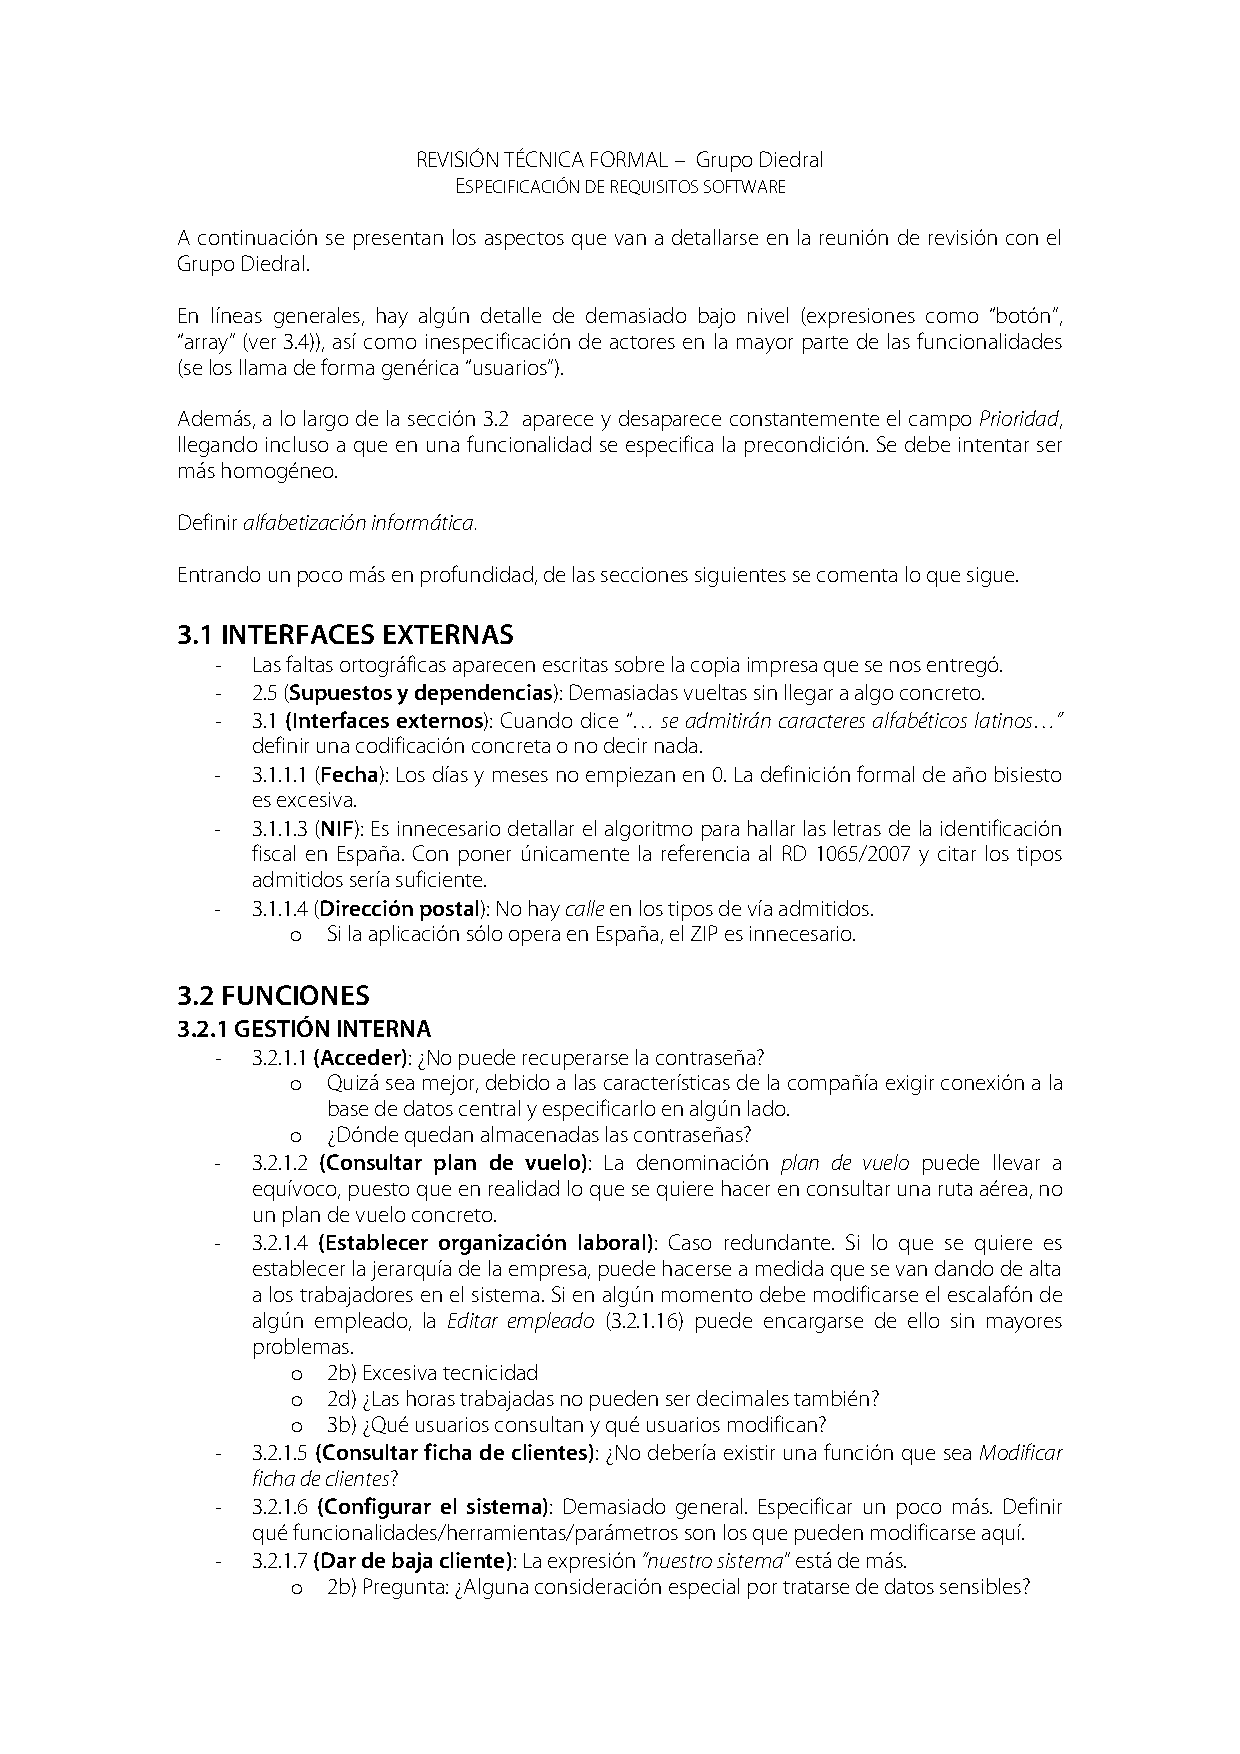
\includepdf[pages=1-2, pagecommand={}]{revsrs_anexo.pdf}
\end{document}
